\chapter{Introduzione all'IA}
\begin{flushright}\small\textit{Lezione 1 -- 24/02/2026 -- Russell \& Norvig, Cap.\ 1 (1.1--1.5)}\end{flushright}


\section{Che cos'\`e l'Intelligenza Artificiale?}
\begin{defbox}[Definizione]
L'\textbf{Intelligenza Artificiale} \`e la disciplina che studia la costruzione di \emph{entit\`a intelligenti}: macchine in grado di \textbf{calcolare come agire efficacemente e in modo sicuro} in un'ampia variet\`a di situazioni nuove.
\end{defbox}

L'IA \`e uno dei campi pi\`u interessanti e in rapida crescita di oggi, con un fatturato annuale superiore a \textbf{mille miliardi di dollari}. Abbraccia una vasta variet\`a di sottocampi: apprendimento, ragionamento, percezione, giochi, dimostrazione di teoremi, guida autonoma, diagnostica medica e molto altro.

Storicamente, la ricerca sull'IA ha seguito quattro grandi approcci, incrociando due dimensioni:
\begin{itemize}
    \item \textbf{Umano vs.\ Razionale}: la macchina deve imitare le prestazioni umane o perseguire una razionalit\`a astratta (fare la ``cosa giusta'')?
    \item \textbf{Pensiero vs.\ Comportamento}: ci si concentra sui processi mentali interni o sul comportamento osservabile?
\end{itemize}

\begin{center}
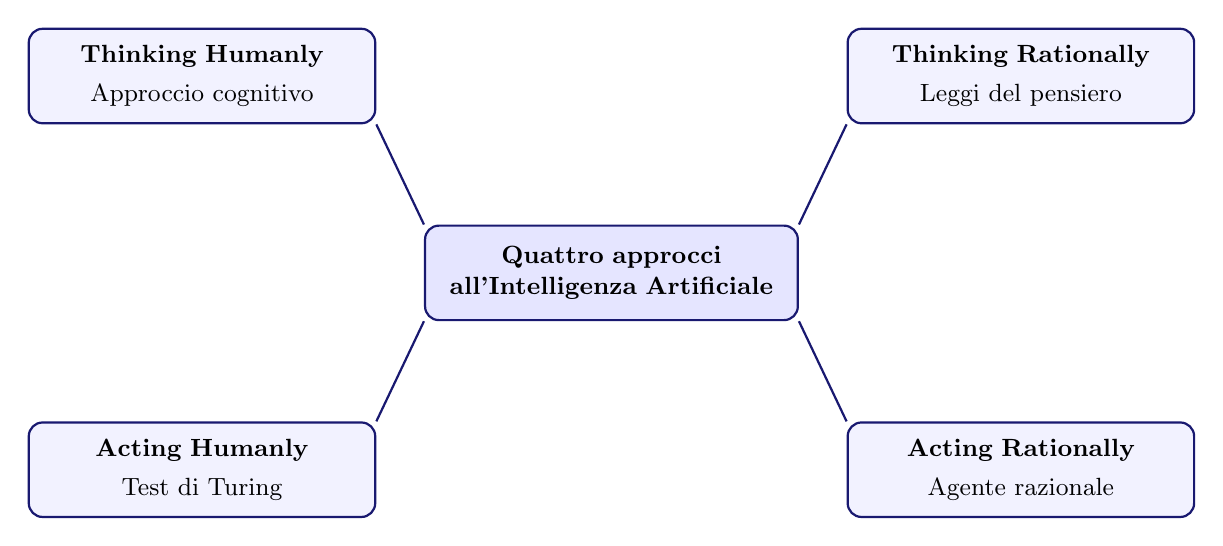
\begin{tikzpicture}[font=\small]
  % Nodo centrale
  \node[
    draw=MidnightBlue, fill=blue!10, thick, rounded corners=5pt,
    minimum width=4.4cm, minimum height=1.2cm, align=center, text width=4.5cm
  ] (center) at (0,0)
  {\bfseries Quattro approcci\\all'Intelligenza Artificiale};

  % Quattro nodi periferici
  \node[
    draw=MidnightBlue, fill=blue!5, thick, rounded corners=5pt,
    minimum width=4.4cm, minimum height=1.2cm, align=center, text width=3.6cm
  ] (TH) at (-5.2, 2.5)
  {\bfseries Thinking Humanly\\[3pt]\normalfont Approccio cognitivo};

  \node[
    draw=MidnightBlue, fill=blue!5, thick, rounded corners=5pt,
    minimum width=4.4cm, minimum height=1.2cm, align=center, text width=3.6cm
  ] (TR) at (5.2, 2.5)
  {\bfseries Thinking Rationally\\[3pt]\normalfont Leggi del pensiero};

  \node[
    draw=MidnightBlue, fill=blue!5, thick, rounded corners=5pt,
    minimum width=4.4cm, minimum height=1.2cm, align=center, text width=3.6cm
  ] (AH) at (-5.2, -2.5)
  {\bfseries Acting Humanly\\[3pt]\normalfont Test di Turing};

  \node[
    draw=MidnightBlue, fill=blue!5, thick, rounded corners=5pt,
    minimum width=4.4cm, minimum height=1.2cm, align=center, text width=3.6cm
  ] (AR) at (5.2, -2.5)
  {\bfseries Acting Rationally\\[3pt]\normalfont Agente razionale};

  % Connessioni
  \draw[thick, MidnightBlue] (TH.south east) -- (center.north west);
  \draw[thick, MidnightBlue] (TR.south west) -- (center.north east);
  \draw[thick, MidnightBlue] (AH.north east) -- (center.south west);
  \draw[thick, MidnightBlue] (AR.north west) -- (center.south east);
\end{tikzpicture}
\end{center}


\subsection{Approccio 1 -- Acting Humanly: il Test di Turing}
\textbf{Alan Turing} (1950) propose un esperimento mentale: un computer supera il test se un interrogatore umano, dopo aver posto domande scritte, non riesce a distinguere le risposte di una macchina da quelle di una persona.

Per superare il test una macchina deve possedere:
\begin{enumerate}
    \item \textbf{Natural Language Processing (NLP)}: comunicare con successo in linguaggio umano.
    \item \textbf{Knowledge Representation}: memorizzare ci\`o che percepisce o apprende.
    \item \textbf{Automated Reasoning}: usare le informazioni salvate per rispondere e trarre conclusioni.
    \item \textbf{Machine Learning}: adattarsi a nuove circostanze e rilevare pattern.
\end{enumerate}

Il \emph{Total Turing Test} aggiunge un segnale video, richiedendo anche \textbf{Computer Vision} e \textbf{Robotica}. Nonostante la sua eleganza, i ricercatori preferiscono studiare i principi sottostanti dell'intelligenza piuttosto che ottimizzare il superamento del test.

\begin{notebox}[L'argomento della stanza cinese (Searle, 1980)]
Superare il test non implica \emph{capire}: un programma potrebbe manipolare simboli senza comprensione, come un uomo chiuso in una stanza che traduce ideogrammi cinesi seguendo manuali senza conoscere la lingua.
\end{notebox}


\subsection{Approccio 2 -- Thinking Humanly: la modellazione cognitiva}
Per dire che un programma ``pensa come un umano'' bisogna prima capire come gli umani pensano. Tre metodi:
\begin{itemize}
    \item \textbf{Introspezione}: osservare i propri pensieri mentre accadono.
    \item \textbf{Esperimenti psicologici}: osservare persone che svolgono compiti e confrontare il loro comportamento con programmi per computer.
    \item \textbf{Brain imaging}: osservare il cervello in azione (fMRI, EEG, MEG).
\end{itemize}

La \textbf{scienza cognitiva} combina modelli computazionali dell'IA con tecniche sperimentali della psicologia per costruire teorie precise e verificabili della mente umana.
L'obiettivo è capire gli schemi mentali umani per riprodurli. Si basa su introspezione, esperimenti psicologici e brain imaging.


\subsection{Approccio 3 -- Thinking Rationally: le leggi del pensiero}
Aristotele fu tra i primi a codificare il ``pensiero corretto'' tramite i \textbf{sillogismi} (``Socrate \`e un uomo; tutti gli uomini sono mortali; quindi Socrate \`e mortale''). Nel XIX secolo i logici svilupparono notazioni precise per ragionare su oggetti e relazioni.

\begin{itemize}
    \item \textbf{Logica formale} (Boole 1847, Frege 1879): fondamento del ragionamento deduttivo in IA.
    \item \textbf{Teoria della probabilit\`a} (Bayes, Laplace): estende la logica al ragionamento in condizioni di incertezza. (C'\`e il 30\% di probabilit\`a di pioggia)
\end{itemize}

Due ostacoli principali: \`e difficile tradurre la conoscenza informale in notazione formale e  molti problemi, anche con pochi fatti, risultano intrattabili.


\subsection{Approccio 4 -- Acting Rationally: l'agente razionale}
\begin{defbox}[Agente razionale]
Un \textbf{agente} \`e un'entit\`a che agisce. Gli agenti software operano \emph{autonomamente}, \emph{percepiscono l'ambiente}, \emph{persistono nel tempo}, \emph{si adattano al cambiamento} e \emph{perseguono obiettivi}.

Un \textbf{agente razionale} agisce in modo da ottenere il \emph{miglior risultato atteso}, anche in condizioni di incertezza.
\end{defbox}

Questo approccio \`e \textbf{pi\`u generale} del ``pensare razionalmente'': l'inferenza corretta \`e solo uno dei meccanismi per essere razionali. \`E anche pi\`u adatto allo sviluppo scientifico, perch\'e la razionalit\`a \`e definita matematicamente in modo preciso e universale. \`E l'approccio prevalente nell'IA moderna, nella teoria del controllo, nella ricerca operativa, nella statistica e nell'economia.

\begin{notebox}[Il Modello Standard e i suoi limiti]
Il ``Modello Standard'' dell'IA assume che il progettista conosca esattamente la funzione obiettivo. \`E pericoloso: se l'obiettivo \`e mal specificato si ottengono comportamenti indesiderati. Russell propone un modello alternativo: la macchina \`e incerta sull'obiettivo umano e impara a inferirlo.
\end{notebox}


\section{Fondamenti dell'Intelligenza Artificiale}
\subsection{Filosofia}
\begin{itemize}
    \item \textbf{Dualismo} (Cartesio): la mente \`e separata dalla materia fisica ed \`e esente dalle leggi fisiche.
    \item \textbf{Empirismo} (Locke, Hume, Bacon): la conoscenza emerge dall'esperienza sensoriale. ``Nulla \`e nell'intelletto che non sia stato prima nei sensi''.
    \item \textbf{Principio di induzione} (Hume): le regole generali si acquisiscono tramite l'esposizione ripetuta ad associazioni tra elementi.
    \item \textbf{Positivismo logico} (Circolo di Vienna): tutta la conoscenza \`e caratterizzata da teorie logiche collegate a osservazioni sensoriali.
    \item \textbf{Conoscenza e azione}: Aristotele propose che le azioni siano giustificate da connessioni logiche tra obiettivi e conoscenza degli esiti.
\end{itemize}


\subsection{Matematica}
\begin{itemize}
    \item \textbf{Logica formale}: Boole (1847), logica proposizionale; Frege (1879), logica del primo ordine con oggetti e relazioni.
    \item \textbf{Probabilit\`a}: Cardano, Pascal, Bayes, Laplace. La \textbf{regola di Bayes} \`e fondamentale per il ragionamento sotto incertezza in IA.
    \item \textbf{Calcolabilit\`a}: G\"odel (1931), Turing (1936), Church. La \emph{Church--Turing thesis} identifica la calcolabilit\`a con le macchine di Turing. Alcune funzioni non sono calcolabili.
    \item \textbf{Trattabilit\`a}: la distinzione tra crescita polinomiale ed esponenziale \`e fondamentale. Molti problemi di IA sono NP-completi e richiedono un uso attento delle risorse computazionali.
\end{itemize}


\subsection{Economia}
\begin{itemize}
    \item \textbf{Teoria delle decisioni}: combina probabilit\`a e utilit\`a per un framework formale per decisioni sotto incertezza (von Neumann \& Morgenstern, 1944).
    \item \textbf{Teoria dei giochi}: analizza situazioni in cui le decisioni di pi\`u agenti si influenzano reciprocamente. Gli agenti razionali possono adottare strategie randomizzate.
    \item \textbf{Processi decisionali di Markov} (Bellman, 1957): formalizzano i problemi decisionali sequenziali, base del Reinforcement Learning.
    \item \textbf{Satisficing} (Simon): gli umani spesso prendono decisioni ``abbastanza buone'' piuttosto che ottimali -- descrive meglio il comportamento reale.
\end{itemize}


\subsection{Neuroscienze}
Il \textbf{neurone} \`e l'unit\`a base del sistema nervoso: corpo cellulare (soma), dendriti (input) e assone (output). Un neurone si connette con $10$--$100\,000$ altri neuroni alle sinapsi tramite reazioni elettrochimiche. Il cervello umano ha $\sim 10^{11}$ neuroni e $\sim 10^{14}$ sinapsi.

\begin{notebox}[Cervello vs.\ Computer]
Il cervello \`e $10^6$ volte pi\`u lento nel ciclo di clock rispetto a un computer moderno, ma compensa con enorme capacit\`a di storage e connettivit\`a.
\end{notebox}


\subsection{Psicologia}
\begin{itemize}
    \item \textbf{Comportamentismo} (Watson, Skinner): rifiuta l'introspezione; studia solo le relazioni oggettive stimolo--risposta.
    \item \textbf{Psicologia cognitiva} (James, Craik): vede il cervello come un dispositivo di elaborazione dell'informazione. Le percezioni e le azioni sono mediate da rappresentazioni interne.
    \item \textbf{Modello di Craik (1943)}: (1) stimolo $\to$ rappresentazione interna; (2) manipolazione cognitiva; (3) retraduzione in azione.
    \item \textbf{Scienza cognitiva} (1956): combina modelli computazionali e psicologia sperimentale; Miller, Chomsky, Newell \& Simon dimostrarono che i computer possono modellare memoria, linguaggio e ragionamento.
\end{itemize}


\subsection{Ingegneria informatica}
\begin{itemize}
    \item I moderni calcolatori nascono durante la Seconda Guerra Mondiale: \textbf{Colossus} (UK, 1943), \textbf{Z-3} (Zuse, 1941), \textbf{ENIAC} (USA, 1945).
    \item \textbf{Legge di Moore}: la potenza computazionale raddoppia ogni 18 mesi, grazie a questa legge, le prestazioni dei PC sono passate dai megaFLOP (milioni di operazioni in virgola mobile al secondo) agli attuali exaFLOP (miliardi di miliardi di operazioni al secondo).
    \item \textbf{Hardware specializzato}: GPU (NVIDIA), TPU (Google), WSE per l'addestramento di modelli di ML. Dal 2012 al 2018, la potenza per il training \`e cresciuta di $300.000\times$.
    \item \textbf{Quantum computing}: Il bit classico vale o 0 o 1. Il Qubit (bit quantistico), grazie al principio di sovrapposizione, può assumere infiniti valori compresi tra 0 e 1 contemporaneamente.
\end{itemize}


\subsection{Teoria del controllo e cibernetica}
\begin{itemize}
    \item Sistemi di feedback autoregolanti precedono i computer: orologio ad acqua (Ktesibios), regolatore del motore a vapore (Watt), termostato (Drebbel).
    \item \textbf{Teoria del controllo} (Maxwell, Wiener): framework matematico per sistemi che minimizzano l'errore tra stato corrente e stato obiettivo. 
    \item \textbf{Cibernetica} (Wiener, 1948): studia il comportamento finalistico che emerge da meccanismi regolatori in macchine e organismi.
    \item \textbf{Controllo ottimo stocastico}: progetta sistemi che massimizzano una funzione obiettivo nel tempo -- parallelo diretto con l'obiettivo dell'IA.
\end{itemize}


\subsection{Linguistica}


\begin{itemize}
    \item \textbf{Comportamentismo linguistico} (Skinner, 1957): il linguaggio si apprende per associazioni stimolo--risposta.
    \item \textbf{Strutture sintattiche} (Chomsky, 1957): il linguaggio mostra creativit\`a -- i bambini comprendono e producono frasi mai sentite prima. La sintassi formale di Chomsky spieg\`o questo fenomeno e poteva essere programmata.
    \item Linguistica moderna e IA nacquero quasi contemporaneamente, dando origine alla \textbf{linguistica computazionale} e al \textbf{Natural Language Processing}.
    \item Insight chiave: comprendere il linguaggio richiede conoscenza del dominio e del contesto, non solo regole sintattiche -- legato alla \textbf{rappresentazione della conoscenza}.
\end{itemize}


\section{Storia dell'Intelligenza Artificiale}


\subsection{Le origini (1943--1956)}

\begin{itemize}
    \item \textbf{McCulloch \& Pitts (1943)}: primo modello formale del neurone artificiale; qualsiasi funzione calcolabile pu\`o essere computata da reti di neuroni.
    \item \textbf{Hebb (1949)}: regola di apprendimento hebbiano -- ``neurons that fire together wire together''.
    \item \textbf{Turing (1950)}: propone il Turing Test, introduce machine learning e algoritmi genetici.
    \item \textbf{Conferenza di Dartmouth (1956)}: McCarthy, Minsky, Shannon e Rochester organizzano il workshop -- \textbf{nascita ufficiale dell'IA} come campo.
\end{itemize}

\subsection{Entusiasmo e aspettative (1952--1969)}

\begin{itemize}
    \item \textbf{Logic Theorist} (Newell \& Simon, 1956): dimostra teoremi di logica formale; Russell rimase deliziato quando il programma trov\`o una dimostrazione pi\`u breve della sua.
    \item \textbf{General Problem Solver} (anni '60): imita i protocolli umani di problem solving -- primo approccio ``Thinking Humanly''.
    \item \textbf{LISP} (McCarthy, 1958): linguaggio dominante dell'IA per 30 anni.
    \item \textbf{Microworlds} (anni '60): domini limitati (es.\ il blocchi-mondo di SHRDLU) dove il problem solving sembrava richiedere intelligenza.
\end{itemize}

\subsection{Una dose di realt\`a e i primi inverni (1966--1986)}

\begin{itemize}
    \item I sistemi fallivano su problemi pi\`u grandi per \textbf{esplosione combinatoria}: scalare a istanze reali si rivel\`o impraticabile.
    \item \textbf{Minsky \& Papert (1969)}: dimostrano i limiti del percettrone (non pu\`o risolvere XOR) $\to$ blocca la ricerca sulle reti neurali per anni.
    \item \textbf{Rapporto Lighthill (1973)}: critica i fallimenti dell'IA $\to$ taglio dei finanziamenti britannici.
    \item \textbf{Sistemi esperti} (DENDRAL 1969, MYCIN anni '70, R1/XCON 1982): primo successo commerciale -- conoscenza di dominio specifica invece di metodi deboli generali. Ma fragili di fronte a incertezza e casi nuovi $\to$ secondo inverno (fine anni '80).
\end{itemize}

\subsection{Rinascita e Deep Learning (1986--oggi)}

\begin{itemize}
    \item \textbf{Backpropagation} (Rumelhart, Hinton, Williams 1986): ri-scoperta e applicazione a molti problemi di apprendimento.
    \item \textbf{Reti bayesiane} (Pearl, 1988): framework rigoroso per il ragionamento probabilistico.
    \item \textbf{Big Data} (2001--oggi): raddoppiare i dati supera qualsiasi miglioramento algoritmico (Banko \& Brill, 2001).
    \item \textbf{ImageNet 2012}: AlexNet di Hinton segna l'inizio del dominio del \textbf{Deep Learning}.
    \item Pietre miliari recenti: \textbf{AlphaGo} (2016), \textbf{Transformer} (2017), \textbf{GPT-3} e \textbf{AlphaFold} (2020), \textbf{ChatGPT} (2022), multimodalit\`a e agenti autonomi (2024+).
\end{itemize}


\section{Stato dell'arte}


Le pubblicazioni di IA sono aumentate di 20 volte tra il 2010 e il 2019.

\begin{exbox}[Applicazioni reali oggi]
\begin{itemize}
    \item \textbf{Sanit\`a}: diagnosi di malattie, scoperta di farmaci.
    \item \textbf{Guida autonoma}: veicoli STANLEY (DARPA 2005), sistemi Waymo, Tesla.
    \item \textbf{NLP}: traduzione automatica, assistenti vocali, LLM (GPT-4, Gemini, Claude).
    \item \textbf{Scienza}: AlphaFold (DeepMind, 2020) ha risolto la predizione 3D delle proteine.
    \item \textbf{Giochi}: Deep Blue (scacchi, 1997), AlphaGo (Go, 2016), AlphaStar (2019).
    \item \textbf{Spam filtering}: algoritmi di ML classificano un miliardo di messaggi al giorno.
\end{itemize}
\end{exbox}

\begin{itemize}
    \item \textbf{Interpretabilit\`a (xAI)}: i sistemi DL sono spesso \emph{black box}. LIME, SHAP, Grad-CAM tentano di renderli trasparenti.
    \item \textbf{Robustezza}: vulnerabilit\`a a \emph{adversarial examples} e input fuori distribuzione.
    \item \textbf{Generalizzazione}: trasferire la conoscenza da un dominio all'altro rimane difficile.
    \item \textbf{Fairness e bias}: i sistemi di IA possono amplificare i pregiudizi nei dati di addestramento.
    \item \textbf{Consumo energetico}: il training di modelli grandi consuma enormi quantit\`a di energia (GPT-3: $\sim$1287 MWh).
\end{itemize}


\section{Rischi e benefici dell'IA}


\subsection{Il Problema dell'Allineamento dei Valori}

\begin{defbox}[Modello Standard]
Il \textbf{Modello Standard} dell'IA prevede la progettazione di sistemi che raggiungono un obiettivo specificato dall'utente. Assume che possiamo specificare completamente l'obiettivo. In realt\`a, in problemi aperti del mondo reale, questo \`e spesso impossibile.
\end{defbox}

\begin{warnbox}[Value Alignment Problem]
Il \textbf{problema dell'allineamento dei valori} \`e la sfida di garantire che gli obiettivi programmati in una macchina siano \emph{allineati con i valori umani}. Un sistema sufficientemente capace che persegue un obiettivo fisso potrebbe trovare modi inattesi per raggiungerlo
\end{warnbox}

\begin{thmbox}[Verso un'IA provabilmente benefica (Russell, \emph{Human Compatible}, 2019)]
Poich\'e non possiamo trasferire tutti gli obiettivi a una macchina, serve un approccio in cui la macchina persegue i nostri obiettivi \emph{rimanendo incerta su quali siano davvero}. Questo la incentiva a: agire con \textbf{cautela}, chiedere \textbf{permesso} prima di azioni importanti, \textbf{apprendere} le preferenze umane, e \textbf{delegare il controllo} all'uomo in caso di incertezza.
\end{thmbox}

\subsection{Rischi e benefici}

\begin{exbox}[Principali benefici]
\begin{itemize}
    \item \textbf{Sanit\`a}: diagnosi, scoperta di farmaci, medicina personalizzata.
    \item \textbf{Scienza}: accelera la ricerca in fisica, biologia, chimica.
    \item \textbf{Economia}: automazione, ottimizzazione, supporto decisionale.
    \item \textbf{Accessibilit\`a}: strumenti per persone con disabilit\`a, risposta alle emergenze.
\end{itemize}
\end{exbox}

\begin{warnbox}[Principali rischi]
\begin{itemize}
    \item \textbf{Disoccupazione tecnologica}: l'automazione pu\`o eliminare posti di lavoro pi\`u rapidamente di quanto ne crei.
    \item \textbf{Bias e discriminazione}: i sistemi amplificano i pregiudizi nei dati.
    \item \textbf{Disinformazione}: deepfake, testo sintetico e media manipolati diffondono informazioni false su scala.
    \item \textbf{Privacy e sorveglianza}: la raccolta massiva di dati abilita una sorveglianza senza precedenti.
    \item \textbf{Concentrazione del potere}: i benefici dell'IA rischiano di concentrarsi in poche grandi aziende o nazioni.
    \item \textbf{Armi autonome}: sistemi militari basati sull'IA sollevano gravi preoccupazioni etiche ed esistenziali.
\end{itemize}
\end{warnbox}

\begin{itemize}
    \item \textbf{AI Act UE (2024)}: prima regolamentazione orizzontale sull'IA; impone requisiti di trasparenza, robustezza e supervisione umana in base al livello di rischio.
    \item \textbf{Collaborazione interdisciplinare}: informatici, etici, filosofi, scienziati sociali ed esperti di dominio devono lavorare insieme.
    \item \textbf{Ricerca fondamentale}: progressi su interpretabilit\`a, robustezza, fairness e allineamento rimangono essenziali.
\end{itemize}